\section{\instType{} Deployment Considerations}

\ifcase \inst	%iSAMI

    The \instType{}-pH is recommended for use in waters with salinity and pH ranges of 25--40 and 7--9, respectively, at temperatures ranging from 0 to 35\,$\degree$C, and depth to 3\,m.

\or			%SAMI

    The \instType{}-pH is recommended for use in waters with salinity and pH ranges of 25-40 and 7-9, respectively, at temperatures ranging from 0 to 35$\degree$C, and depth to 600\,m.  The \instType{} can be configured to measure waters with lower salinity and pH. High pressure rated versions are also available for deeper deployments.  The \instType{}-pH can support and log data for up to three external instruments, such as PAR, dissolved oxygen, CTD, and chlorophyll fluorometer.  Please contact sales or technical support to discuss these options.

\or			%AFT

The \instType{} is intended for measurements of flow-through seawater from a ship sampling line.  Set up is described in Chapter.  Care must be taken to avoid excessive positive or negative pressure in the \instType{} wet chamber.  Excessive pressure can cause seawater to leak into the electronic chamber, destroying optics and electronics.  Negative pressure can cause air bubbles to form in the optical cell, resulting in poor pH precision. 

The \instType{} is a spectrophotometric instrument which discharges a small amount of dye into the seawater stream.  Any instrument located upstream of the \instType{} in the seawater line should not alter the visible spectrum of the seawater.  Instruments located downstream of the \instType{} should not be affected by the dye.  

pH is reported at the temperature in the wet chamber of the \instType{}.  In order to report pH at in situ temperature, in situ temperature must be measured, and the pH should be corrected using the following equation:

\begin{equation}
pH_{is} = {pH_m} + 0.015 ( T_m - T_{is} )
\end{equation}

where $pH_{is}$ is in situ pH, $pH_m$ is pH measured by the \instType{}, $T_{is}$ is in situ temperature in C, and $T_m$ is measured temperature in C.

\fi


\subsection{pH Range}

The measurable pH range of the \instType{}-pH is dictated by the \pKa{} of the indicator, \textit{meta}-cresol purple (\mCP{}), and is 7--9 in the standard configuration.  Below and above this range, absorbances become unreliable, and accuracy degrades.  Different pH indicators in combination with different optics can be used to target a different pH, but the targeted range will not exceed 2 pH units.  Targeting a pH range other than 7--9 requires using an indicator that is not as well characterized as \mCP{}, and could result in less accurate pH measurement.  Table \ref{pH Measurement Range} summarizes available indicators and their pH ranges at salinity of 35. 

\begin{table}[ht]
   \begin{center}
   \caption{\label{pH Measurement Range}pH Measurement Range\\ $^\ast$at salinity 35 and 15$\degree$C}
   \vspace{3mm}
   \centering
   \begin{tabular}{m{30mm} m{30mm} @{}m{0mm}}
      \toprule
      \centering \textbf{Indicator} & \centering \textbf{pH Range$^\ast$} & \\
      \midrule
      \centering thymol blue & \centering 7.5--9.5 & \\
      \midrule
      \centering \textit{meta}-cresol purple & \centering 7.1--9.1 & \\
      \midrule
      \centering phenol red & \centering 6.5--8.5 & \\   
      \midrule
      \centering bromo-cresol purple & \centering 4.9--6.9 &\\
      \bottomrule
   \end{tabular}
   \end{center}
\end{table}


\subsection{Salinity Range}

The \pKa{} of the indicator is dependent on temperature and salinity, and thus both need to be measured for accurate pH measurement.  If salinity is known to $\pm$\,1\,PSU, using the average, constant salinity to calculate the measured pH is adequate.  If salinity varies at the deployment site, salinity should be measured with an external instrument.  \ifcase \inst {} \or {The salinity logged by a \instType{} that is controlling a CTD can be used with \instType{} Client software to calculate pH. If the CTD } \or {The salinity logged by a \instType{} that is controlling a TSG can be used with \instType{} Client software to calculate pH. If the TSG } \fi logs salinity independently, a standalone Matlab routine can be used to calculate pH with the measured salinity.  

\ifcase \inst	%iSAMI

    \instType{}-pH instruments will be accurate to $\pm$\,0.007\,pH through the salinity range of 25--40.  Limited results from lower salinities have given accuracies better than $\pm$\,0.015\,pH.

\else			%SAMI/AFT

    \instType{}-pH instruments will be accurate to $\pm$\,0.004\,pH through the salinity range of 25--40.  Limited results from lower salinities have given accuracies better than $\pm\,$0.015\,pH.
    
\fi

\ifcase \inst	%iSAMI

\or			%SAMI

\or			%AFT

\subsection{Using the \instType{} to measure the pH of discrete samples}

The \instType{}-pH can be configured by Sunburst Sensors to measure the pH of discrete samples. If you intend to use your \instType{} to measure discrete samples, please contact sales or technical support.  In this configuration, the \instType{} will have an additional 3-way solenoid valve to switch between sampling through the wet chamber and sampling through the tubing that comes out the side of the instrument.  When sampling from the tubing, the sample should be placed in a thermostatted water bath. The water bath should be circulated through the wet chamber of the \instType{}, with care to not apply excessive positive or negative pressure.  The inlet tubing should be placed inside the sample.  Failure to circulate thermostatted water through the wet chamber will result in poor accuracy and precision in the pH measurement, as pH is highly temperature sensitive. Note that when measuring the pH of discrete samples, on the \textbf{Settings} tab,
SAMI/AFT panel, bottle must be chosen by entering a 1 in the box.

\fi


\subsection{Measurement Frequency}

\ifcase \inst	%iSAMI

    \begin{table}[ht]
       \begin{center}
       \caption{\label{Reagent Life}Reagent Life}
       \vspace{3mm}
       \centering
       \begin{tabular}{m{30mm} m{30mm} m{30mm}@{}m{0mm}@{}}
          \toprule
          \centering Measurement\newline interval (min) & \centering Measurement\newline frequency ($\mathrm{d^{-1}}$) & \centering \instType{} total reagent life (d), 200\,mL & \\
          \midrule
          \centering 15 & \centering 96 & \centering 83 & \\
          \midrule
          \centering 30 & \centering 48 & \centering 167 & \\   
          \midrule
          \centering 60 & \centering 24 & \centering 333 &\\
          \midrule
          \centering 120 & \centering 12 & \centering 667 & \\ 
          \bottomrule
       \end{tabular}
       \end{center}
    \end{table}

\else			%SAMI/AFT

   \begin{table}[ht]
       \begin{center}
       \caption{\label{Reagent Life}Reagent Life}
       \vspace{3mm}
       \centering
       \begin{tabular}{m{30mm} m{30mm} m{30mm}@{}m{0mm}@{}}
          \toprule
          \centering Measurement\newline interval (min) & \centering Measurement\newline frequency ($\mathrm{d^{-1}}$) & \centering \instType{} total reagent life (d), 550\,mL & \\
          \midrule
          \centering 15 & \centering 96 & \centering 114 & \\
          \midrule
          \centering 30 & \centering 48 & \centering 229 & \\   
          \midrule
          \centering 60 & \centering 24 & \centering 458 &\\
          \midrule
          \centering 120 & \centering 12 & \centering 916 & \\ 
          \bottomrule
       \end{tabular}
       \end{center}
    \end{table}
\fi

\ifcase \inst	%iSAMI

    \begin{table}[ht]
       \begin{center}
       \caption{\label{Battery Life}Battery Life}
       \vspace{3mm}
       \centering
       \begin{tabular}{m{30mm} m{30mm} m{30mm} @{}m{0mm}@{}}
          \toprule
          \centering Measurement\newline interval (min) & \centering Measurement\newline frequency ($\mathrm{d^{-1}}$) & \centering \instType{} total battery life* (d), 0\,$\degree$C & \\
          \midrule
          \centering 15 & \centering 96 & \centering 87 & \\
          \midrule
          \centering 30 & \centering 48 & \centering 174 & \\
          \midrule
          \centering 60 & \centering 24 & \centering 349 & \\
          \midrule
          \centering 120 & \centering 12 & \centering 697& \\
          \bottomrule
       \end{tabular}
       \end{center}
    \end{table}

\else			%SAMI/AFT

    \begin{table}[ht]
       \begin{center}
       \caption{\label{Battery Life}Battery Life}
       \vspace{3mm}
       \centering
       \begin{tabular}{m{30mm} m{30mm} m{30mm} @{}m{0mm}@{}}
          \toprule
          \centering Measurement\newline interval (min) & \centering Measurement\newline frequency ($\mathrm{d^{-1}}$) & \centering \instType{} total battery life* (d), 0\,$\degree$C & \\
          \midrule
          \centering 15 & \centering 96 & \centering 58 & \\
          \midrule
          \centering 30 & \centering 48 & \centering 117 & \\
          \midrule
          \centering 60 & \centering 24 & \centering 234 & \\
          \midrule
          \centering 120 & \centering 12 & \centering 468 & \\
          \bottomrule
       \end{tabular}
       \end{center}
    \end{table}
    
\fi

By collecting a higher quantity of data points you will more quickly use reagent, battery life, and memory, which will shorten the longevity of your collection time. We encourage you to weigh your options to maximize the effectiveness of your deployment while considering the questions you are trying to answer through your research. Use the tables included above to help you decide upon the appropriate parameters for your deployment.


\ifcase \inst	%iSAMI

\subsection{Cold Water Deployment}

The \instType{}-pH indicator contains NaCl equal to salinity 35, which will prevent the indicator from freezing in seawater.  However, water or indicator inside the narrow gauge tubing will freeze quickly if the \instType{} is kept at below-freezing temperatures for very long.  This will result in loss of data until ice within the tubing melts.  If you are planning to deploy your \instType{}-pH in below-freezing weather, we recommend that you take the following precautions to avoid data loss:

\begin{enumerate}
\item
Remove the copper bell attached to the sample inlet \ifcase \inst {tube.} \or {tube (this tube extrudes from and is zip-tied to the brass cage).} \fi Ice can form around the copper bell if it has water in it.
\item
Please let the sales or technical staff at Sunburst know about the cold weather deployment, and request a blank bag with 10\,\% ethylene glycol. Ethylene glycol will decrease the freezing temperature of the water in the bag.
\item
Minimize the amount of time that your \instType{}-pH is exposed to cold weather before deploying.
\end{enumerate}

\or			%SAMI

\subsection{Cold Water Deployment}

The \instType{}-pH indicator contains NaCl equal to salinity 35, which will prevent the indicator from freezing in seawater.  However, water or indicator inside the narrow gauge tubing will freeze quickly if the \instType{} is kept at below-freezing temperatures for very long.  This will result in loss of data until ice within the tubing melts.  If you are planning to deploy your \instType{}-pH in below-freezing weather, we recommend that you take the following precautions to avoid data loss:

\begin{enumerate}
\item
Remove the copper bell attached to the sample inlet \ifcase \inst {tube.} \or {tube (this tube extrudes from and is zip-tied to the brass cage).} \fi Ice can form around the copper bell if it has water in it.
\item
Please let the sales or technical staff at Sunburst know about the cold weather deployment, and request a blank bag with 10\,\% ethylene glycol. Ethylene glycol will decrease the freezing temperature of the water in the bag.
\item
Minimize the amount of time that your \instType{}-pH is exposed to cold weather before deploying.
\end{enumerate}

\or			%AFT

\fi


\ifcase \inst	%iSAMI

\subsection{Deployment in High TDS or Highly Productive Areas}

The \instType{}-pH pumps about 3\,mL of seawater through the system for every pH measurement.  The hardware can become clogged or malfunctional and optical throughput can degrade due to fine particles or biological fouling.  An inlet filter was shipped with your \instType{}-pH.  Use the following guide to decide whether to use it.

\textbf{Use the inlet filter} if you will be deploying in a high fouling or silty area.  Be advised that this might cause some degree of resolution loss if the pH is highly variable.  You can increase the number of flush pumps if necessary, although this will decrease battery life.  We believe that it might be necessary to change the filter during deployment if it becomes highly fouled, but we cannot give advice as to how long the filter will work for.  Order extra filters if you think you will need them.

\textbf{Use the copper bell} if you are not concerned about fouling due to deep, cold, or non-productive water.  You can also deploy with the copper bell (without the filter) if you want to be sure to completely resolve pH when it is rapidly changing,  Be advised that the \instType{} might foul after a month or two and begin to give erratic data if the water is highly productive.

\textbf{Remove the copper bell} if you are deploying in cold temperatures and are concerned about the \instType{} fluids freezing during the time that the \instType{} is exposed to freezing temperatures prior to deployment.

Refer to Figure \ref{fig:FilterFig}  when following instructions for \instType{} inlet configuration.


\subsubsection{Instructions for inlet filter use}

\begin{enumerate}
\item
Unscrew the white union inside the copper bell (A).
\item
Approximately 1 inch of tubing will protrude from the blue nut (B).  The copper bell can be left on or removed.
\item 
The filter is pre-wetted with isopropyl alcohol.  It is shipped with a small amount of deionized water to deep it wet, but there may be a residual amount of alcohol in the bag (C).
\item
Insert the tubing into the filter and connect using the blue nut.  The tubing will go all the way to the bottom of the filter (D).
\item
Remove the blank bag by cutting the zip tie.  A plug for the bag is included with the flushing syringe (E).
\item
Secure the filter with a zip tie before deployment (E).
\end{enumerate}


\subsubsection{Instructions for copper bell use}

\begin{enumerate}
\item
Unscrew the white union inside the copper bell (A).
\item
Approximately 1 inch of tubing will protrude from the blue nut (B).
\item
Using a razor or other sharp edge, cut the tubing flush with the blue nut, being careful to not crimp the tubing end (F).
\item
Remove the blank bag by cutting the zip tie (E).  A plug for the bag is included with the flushing syringe.
\end{enumerate}


\subsubsection{Instructions for bare tubing use}

\begin{enumerate}
\item
Unscrew the white union inside the copper bell (A).
\item
Approximately 1 inch of tubing will protrude from the blue nut (B).
\item
Unscrew the copper bell (G).
\item
Using a razor or other sharp edge, cut the tubing flush with the blue nut, being careful to not crimp the tubing end (G).
\item
Remove the blank bag by cutting the zip tie (E).  A plug for the bag is included with the flushing syringe.
\end{enumerate}

\begin{figure}
\centering
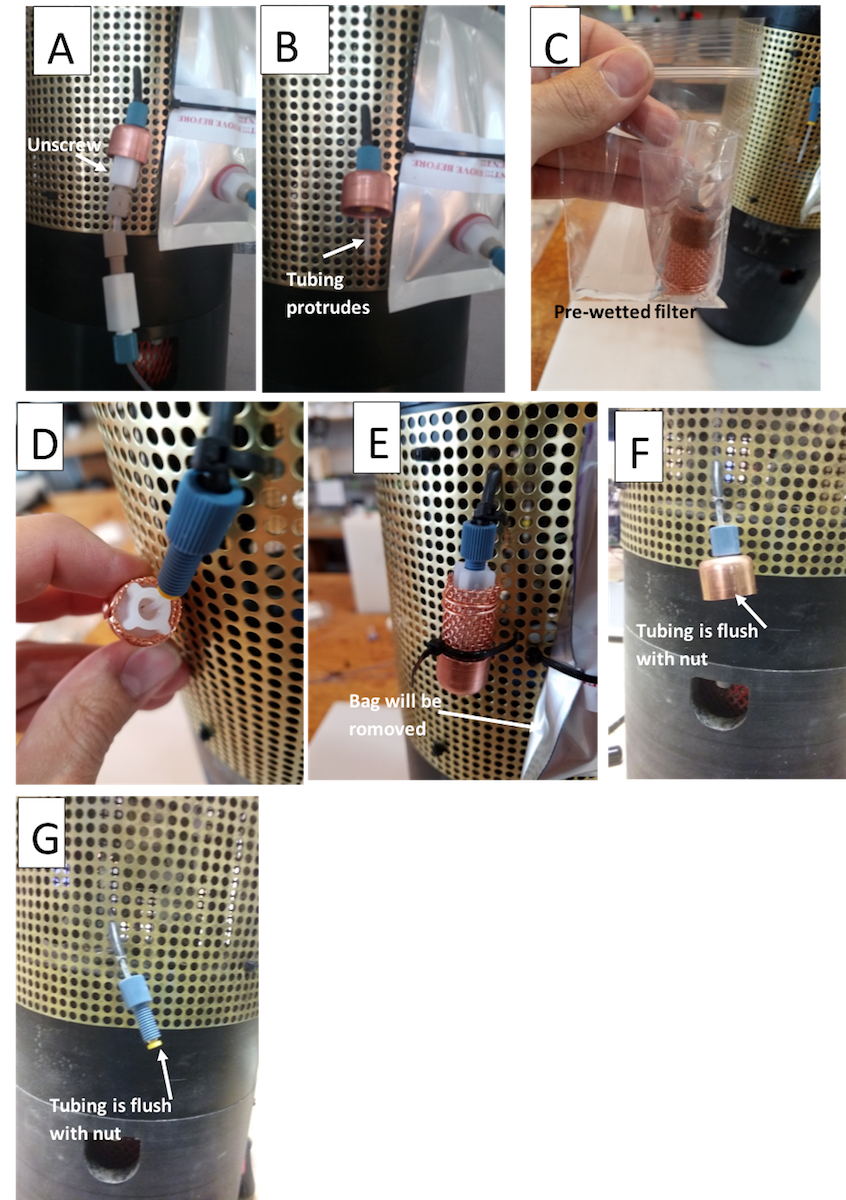
\includegraphics[width=1.0\textwidth]{figs/Filter_Fig.png}
\caption{\instType{} inlet configuration}
\label{fig:FilterFig}
\end{figure}

\or		%SAMI

\subsection{Deployment in High TDS or Highly Productive Areas}

The \instType{}-pH pumps about 1\,mL of seawater through the system for every pH measurement.  The hardware can become clogged or malfunctional and optical throughput can degrade due to fine particles or biological fouling.  An inlet filter was shipped with your \instType{}-pH.  Use the following guide to decide whether to use it.  If you are concerned about the \instType{} failing due to highly productive or silty water, please contact technical support to request an inlet filter.  This filter will cause loss of resolution and will require more pumping, which will drain the battery faster.

\textbf{Use the inlet filter} if you will be deploying in a high fouling or silty area.  Be advised that this might cause some degree of resolution loss if the pH is highly variable.  You can increase the number of flush pumps if necessary, although this will decrease battery life.  We believe that it might be necessary to change the filter during deployment if it becomes highly fouled, but we cannot give advice as to how long the filter will work for.  Order extra filters if you think you will need them.

\textbf{Use the copper bell} if you are not concerned about fouling due to deep, cold, or non-productive water.  You can also deploy with the copper bell (without the filter) if you want to be sure to completely resolve pH when it is rapidly changing,  Be advised that the \instType{} might foul after a month or two and begin to give erratic data if the water is highly productive.

\textbf{Remove the copper bell} if you are deploying in cold temperatures and are concerned about the \instType{} fluids freezing during the time that the \instType{} is exposed to freezing temperatures prior to deployment.

Refer to Figure \ref{fig:FilterFig}  when following instructions for \instType{} inlet configuration.


\subsubsection{Instructions for inlet filter use}

\begin{enumerate}
\item
Unscrew the white union inside the copper bell (A).
\item
Approximately 1 inch of tubing will protrude from the blue nut (B).  The copper bell can be left on or removed.
\item 
The filter is pre-wetted with isopropyl alcohol.  It is shipped with a small amount of deionized water to deep it wet, but there may be a residual amount of alcohol in the bag (C).
\item
Insert the tubing into the filter and connect using the blue nut.  The tubing will go all the way to the bottom of the filter (D).
\item
Remove the blank bag by cutting the zip tie.  A plug for the bag is included with the flushing syringe (E).
\item
Secure the filter with a zip tie before deployment (E).
\end{enumerate}


\subsubsection{Instructions for copper bell use}

\begin{enumerate}
\item
Unscrew the white union inside the copper bell (A).
\item
Approximately 1 inch of tubing will protrude from the blue nut (B).
\item
Using a razor or other sharp edge, cut the tubing flush with the blue nut, being careful to not crimp the tubing end (F).
\item
Remove the blank bag by cutting the zip tie (E).  A plug for the bag is included with the flushing syringe.
\end{enumerate}


\subsubsection{Instructions for bare tubing use}

\begin{enumerate}
\item
Unscrew the white union inside the copper bell (A).
\item
Approximately 1 inch of tubing will protrude from the blue nut (B).
\item
Unscrew the copper bell (G).
\item
Using a razor or other sharp edge, cut the tubing flush with the blue nut, being careful to not crimp the tubing end (G).
\item
Remove the blank bag by cutting the zip tie (E).  A plug for the bag is included with the flushing syringe.
\end{enumerate}

\begin{figure}
\centering
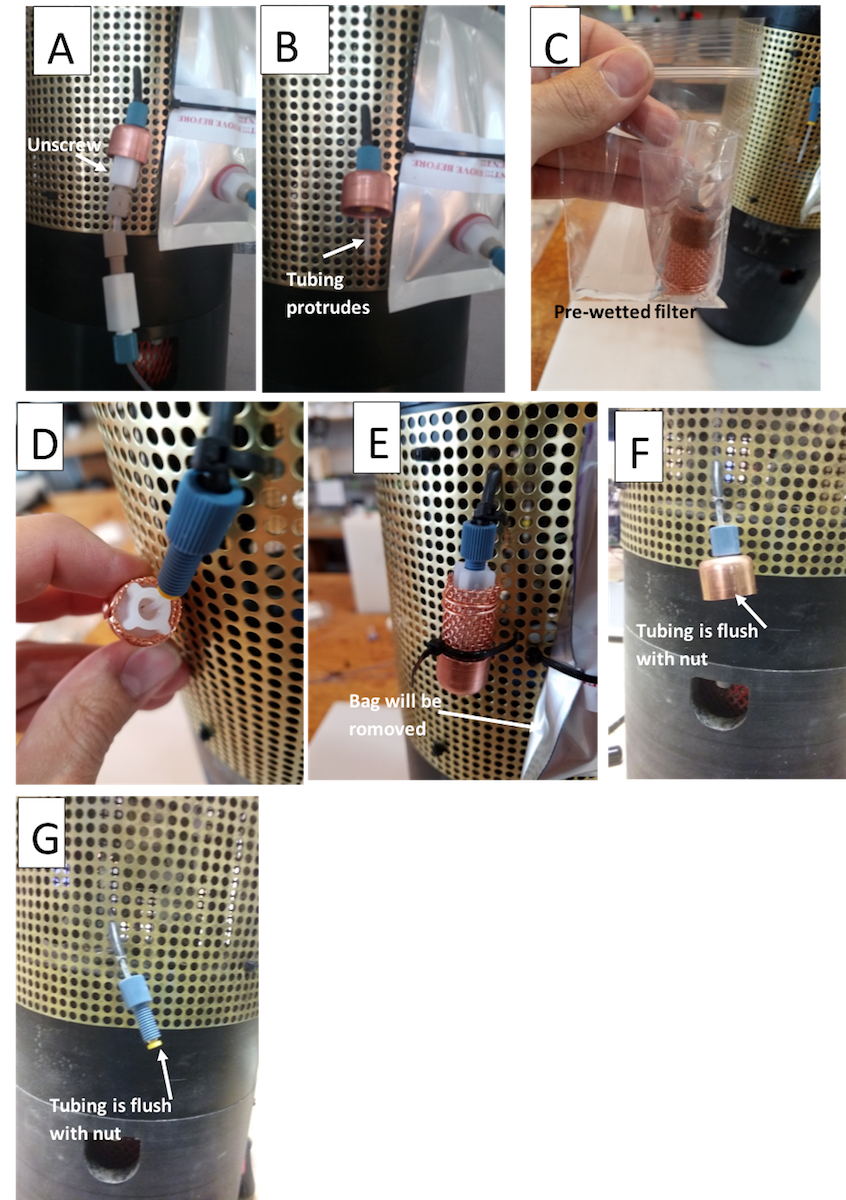
\includegraphics[width=1.0\textwidth]{figs/Filter_Fig.png}
\caption{\instType{} inlet configuration}
\label{fig:FilterFig}
\end{figure}


\subsection{Avoiding Air-Lock}

Care must be taken to avoid deploying the \instType{}-pH with air in the tubing, or pumping the \instType{} when it is not either connected to the blank bag or immersed in water.  If the \instType{} tubing is full of air when it is deployed, this can cause the pumps to lock up, and no useful data will be collected.  

Before deploying the \instType{}-pH, flush with blank.  Leave the blank bag connected to the inlet and perform a pH flush using the \instType{} client software as described in section \ref{sec:AirLock}.  After flushing is complete, set the sample start to a time well after deployment is expected. Be sure to remove the blank bag from the inlet before deploying.

\fi